\documentclass[12pt, letterpaper]{article}
\usepackage[utf8]{inputenc}
\usepackage{graphicx}

\renewcommand*\contentsname{Indholdsfortegnelse}



\begin{document}

\begin{titlepage}

\newcommand{\HRule}{\rule{\linewidth}{0.5mm}} % Defines a new command for the horizontal lines, change thickness here

\center % Center everything on the page
 
%----------------------------------------------------------------------------------------
%	HEADING SECTIONS
%----------------------------------------------------------------------------------------

\textsc{\LARGE Aarhus universitet}\\[1.5cm] % Name of your university/college
\textsc{\Large KVI}\\[0.5cm] % Major heading such as course name
\textsc{\large Semester 3}\\[0.5cm] % Minor heading such as course title

%----------------------------------------------------------------------------------------
%	TITLE SECTION
%----------------------------------------------------------------------------------------

\HRule \\[0.4cm]
{ \huge \bfseries NOTER}\\[0.4cm] % Title of your document
\HRule \\[1.5cm]
 
%----------------------------------------------------------------------------------------
%	AUTHOR SECTION
%----------------------------------------------------------------------------------------

% If you don't want a supervisor, uncomment the two lines below and remove the section above
\Large \emph{Studerende:}\\[1cm]
Mette \textsc{Hammer Nielsen-Kudsk}\\[0,5cm] % Your name
Martin \textsc{Banasik}\\[1cm] % Your name
%----------------------------------------------------------------------------------------
%	DATE SECTION
%----------------------------------------------------------------------------------------

{\large \today}\\[1,2cm] % Date, change the \today to a set date if you want to be precise

%----------------------------------------------------------------------------------------
%	LOGO SECTION
%----------------------------------------------------------------------------------------


\includegraphics[scale=0.5]{billeder/au}\\ % Include a department/university logo - this will require the graphicx package
 
%----------------------------------------------------------------------------------------

\vfill % Fill the rest of the page with whitespace


\end{titlepage}
\tableofcontents
\newpage

\section{Biostatistik}

Variationer når man begynder at måle.
Systematisk variation
\begin{itemize}
\item Mænd er højere end kvinder
\item Blodtrykket stiger med alderen
\item Rygning øger risikoen for lunge cancer \newline


Tilfældig variation

\item Analytisk variation (målefejl)
\item Biologisk variation
\item Observatør variation (rapportering)
\end{itemize}

\subsection{Hvorfor statistik?}
\begin{itemize}
\item Behov for at kvantificere hvor meget af den observerede data der skyldes tilfældige variation og hvor meget der skyldes systematisk variation. \newline
\item Behov for at resumere mange enkelte observationer i nogle få tal.
\end{itemize}
\subsection{Hvorfor stikprøver (samples)?}
\begin{itemize}
\item Hurtigere, billigere, umligt at undersøge alle, kan være tilstrækkelig med en sample, statisktiske metoder kan bruges til at vurdere usikkerhed. \newline

Dataanalysen kan opdeles i \newline
\textsc {Deskriptiv statistik}
Som er et data summary. Indeholder:
\item gennemsnit / median / percentiler
\item hyppigheder / relativ risiko / oddsratio
\item Tegninger/figurer - Vigtig! \newline

\textsc{statisktisk inferens}
\item Model / antagelser angående variationen i data
\item Estimation af relevante parametre i modellen (sample fra populationen) ( f.eks. middelværdi eller forskel mellem to grupper) ud fra stikprøven med tilgørende sikkerhedsintervaller
\item Opstilling af statisktiske hypoteser, statistiske test
\item Statiske konklusioner
\item Kvantificere usikkerheden på estimatet
\item Faglige konklusioner
\end{itemize}

\textsc{statisktisk inferens}
\begin{itemize}
\item Kvalitative data (kategoriske data)
\begin{itemize}
\item F.eks. køn, blodtype (ABO)
\end{itemize}
\item Kvantitative data (numeriske data)
\begin{itemize}
\item F.eks fødselsvægt, blodtryk, cancer incidens
\end{itemize}
\item Diskrete data
\begin{itemize}
\item Når observationer kun kna antage visse numeriske værdier
\end{itemize}
\item Kontinuære data
\begin{itemize}
\item Som regel ved måling, f.eks FEV1, SVR
\end{itemize}
\end{itemize}

\begin{center}
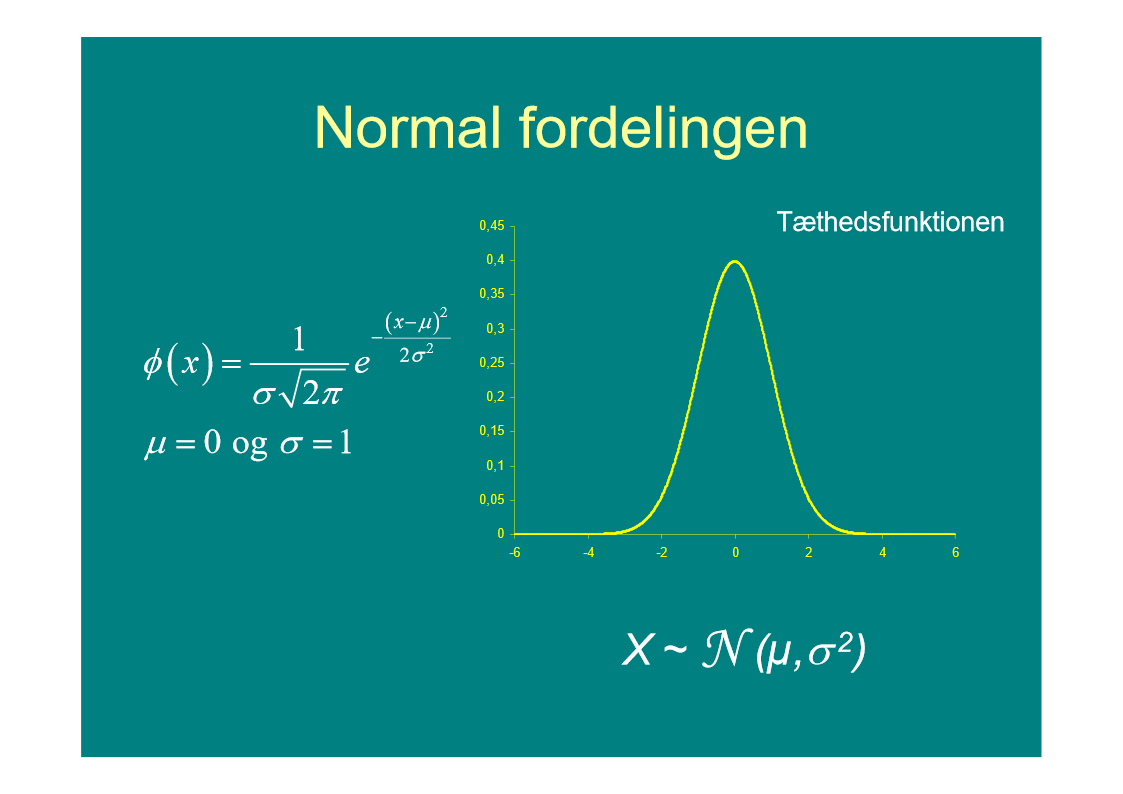
\includegraphics[width=\textwidth]{billeder/billede21}
\end{center}
Normal fordelingen. Klokkeform. Spredningen er = 1 og middelværdi er = 0

\begin{center}
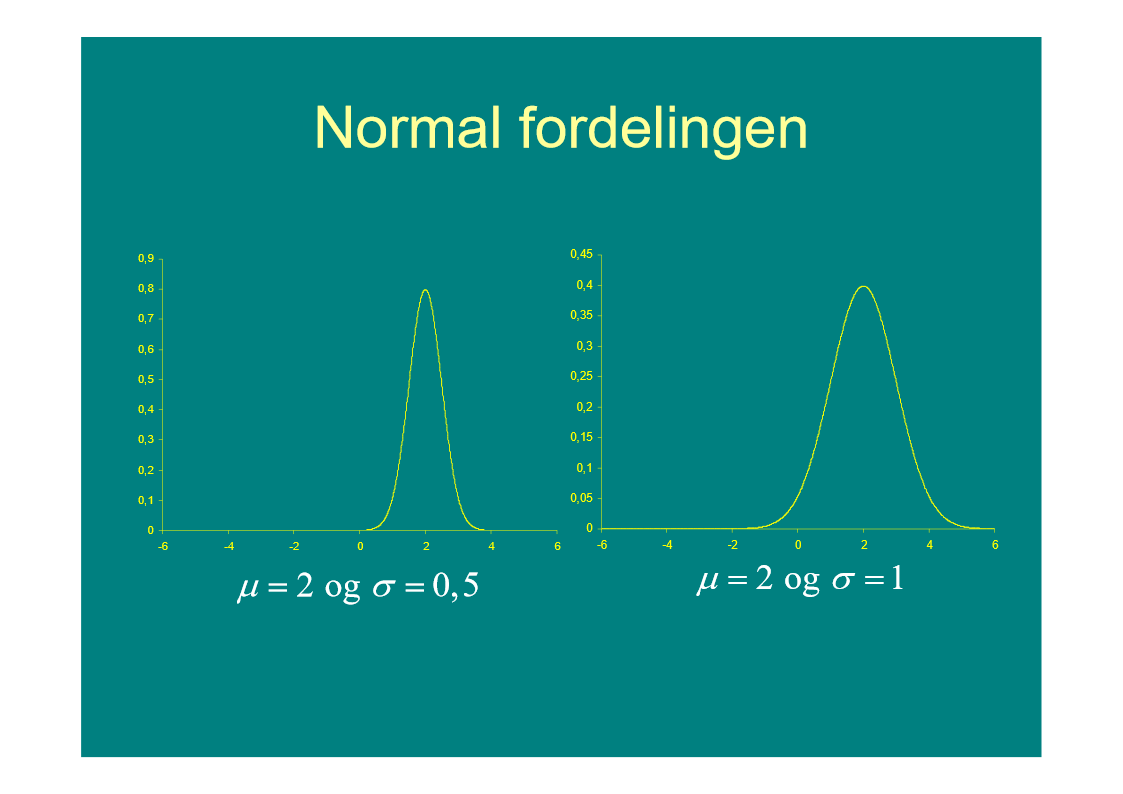
\includegraphics[width=\textwidth]{billeder/billede22}
\end{center}
Til venstre viser den en middelværdi = 2 og en spredning = 0,5. til højre er middelværdi = 2 og en spredning = 1. 

Middelværdien viser placeringen og spredningen viser breden af klokkeformen. 

\begin{center}
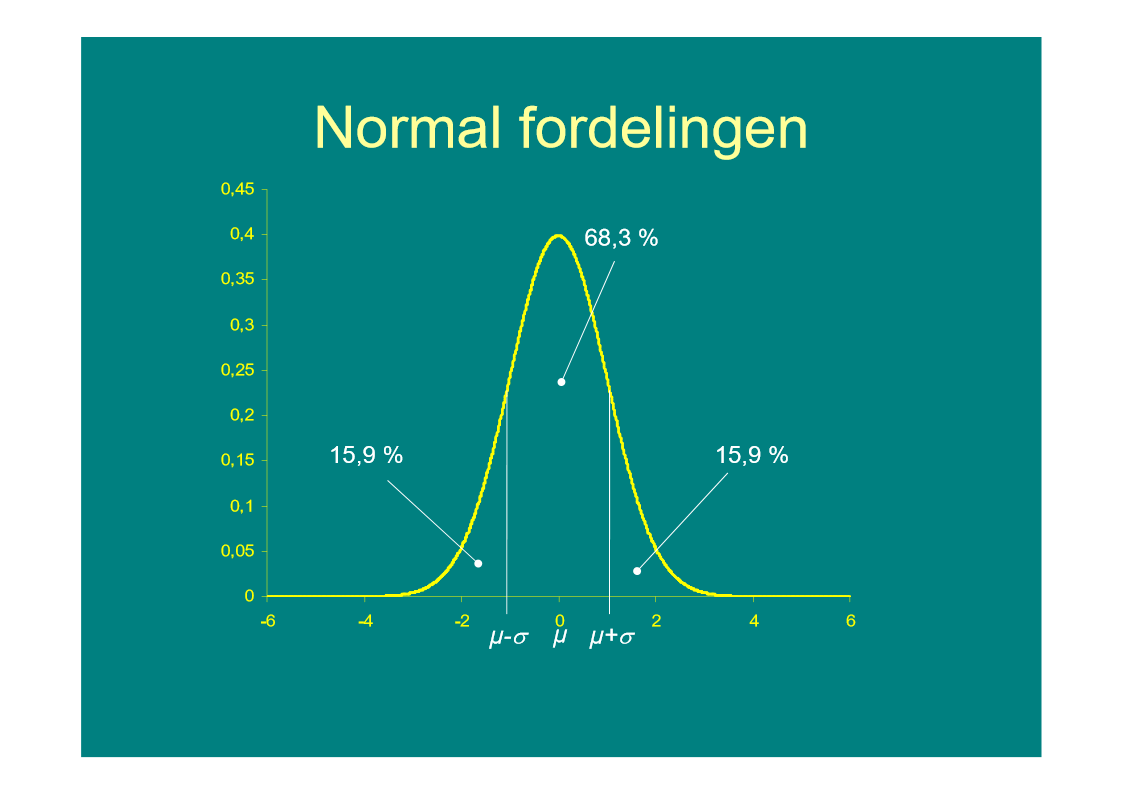
\includegraphics[width=\textwidth]{billeder/billede23}
\end{center}

\begin{center}
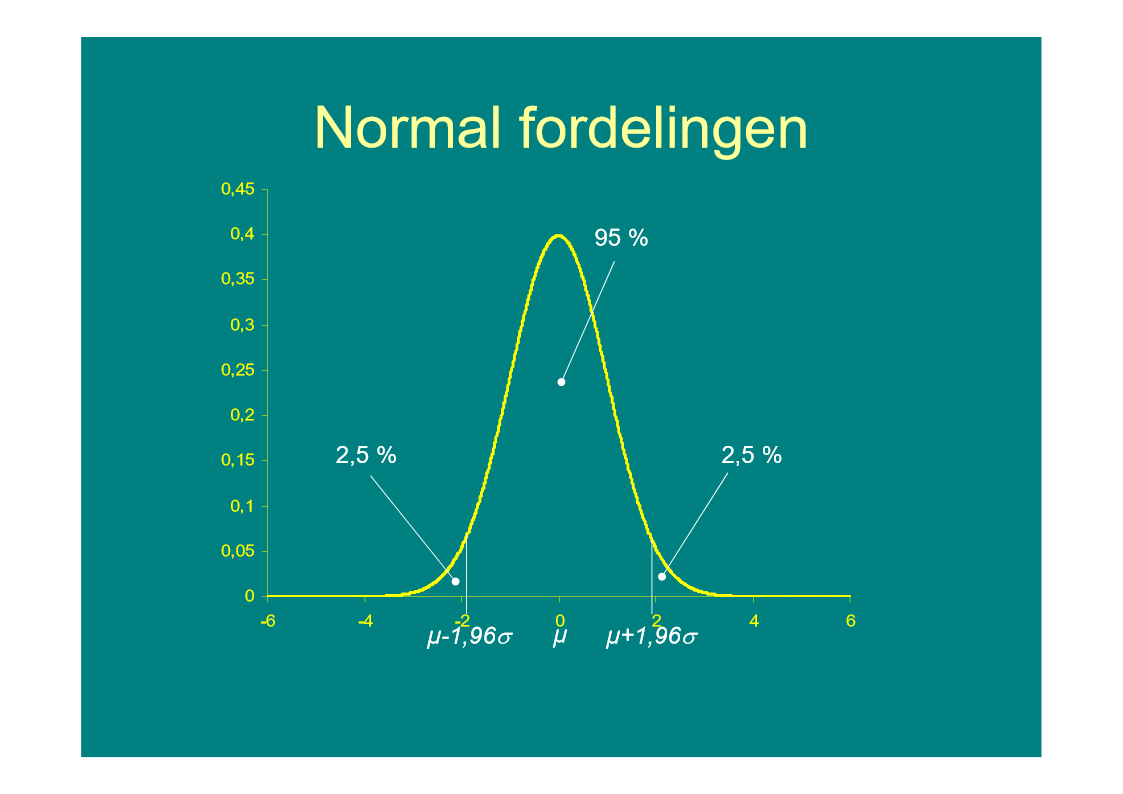
\includegraphics[width=\textwidth]{billeder/billede24}
\end{center}
Beskriver hvor meget vores data spreder sig. En lille spredning er lig færre stikprøver.

\begin{center}
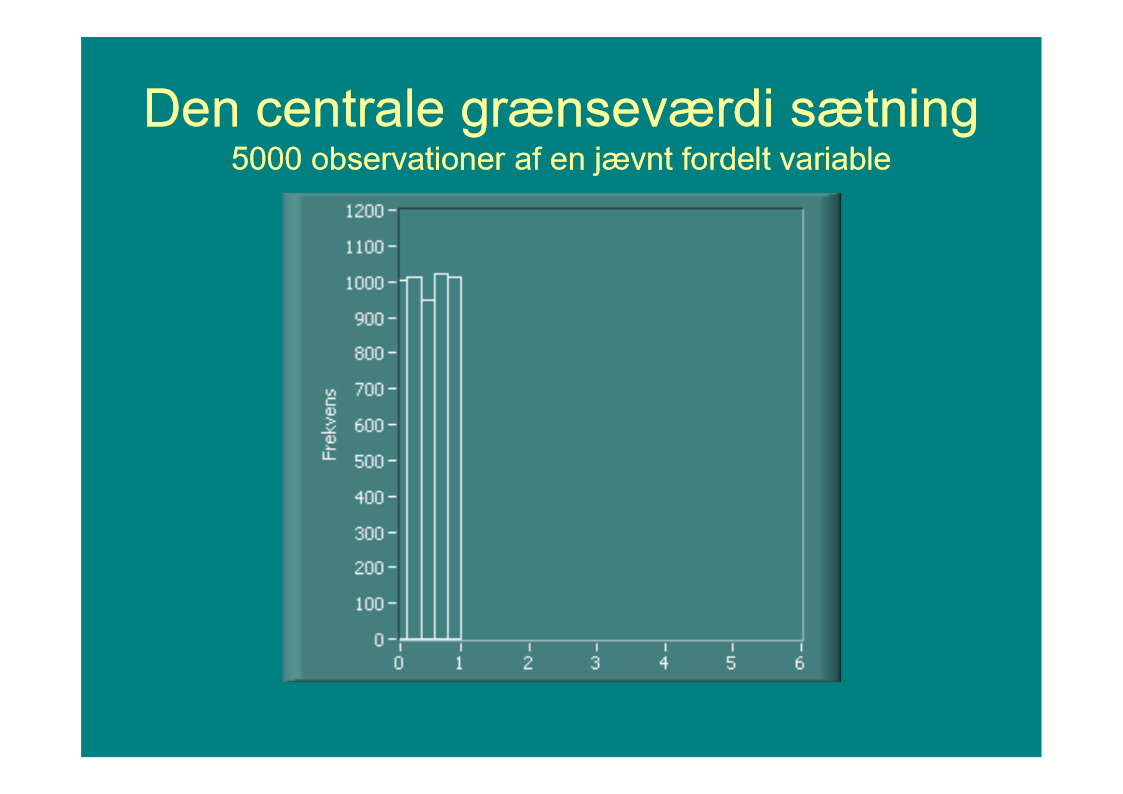
\includegraphics[width=\textwidth]{billeder/billede25}
\end{center}

\begin{center}
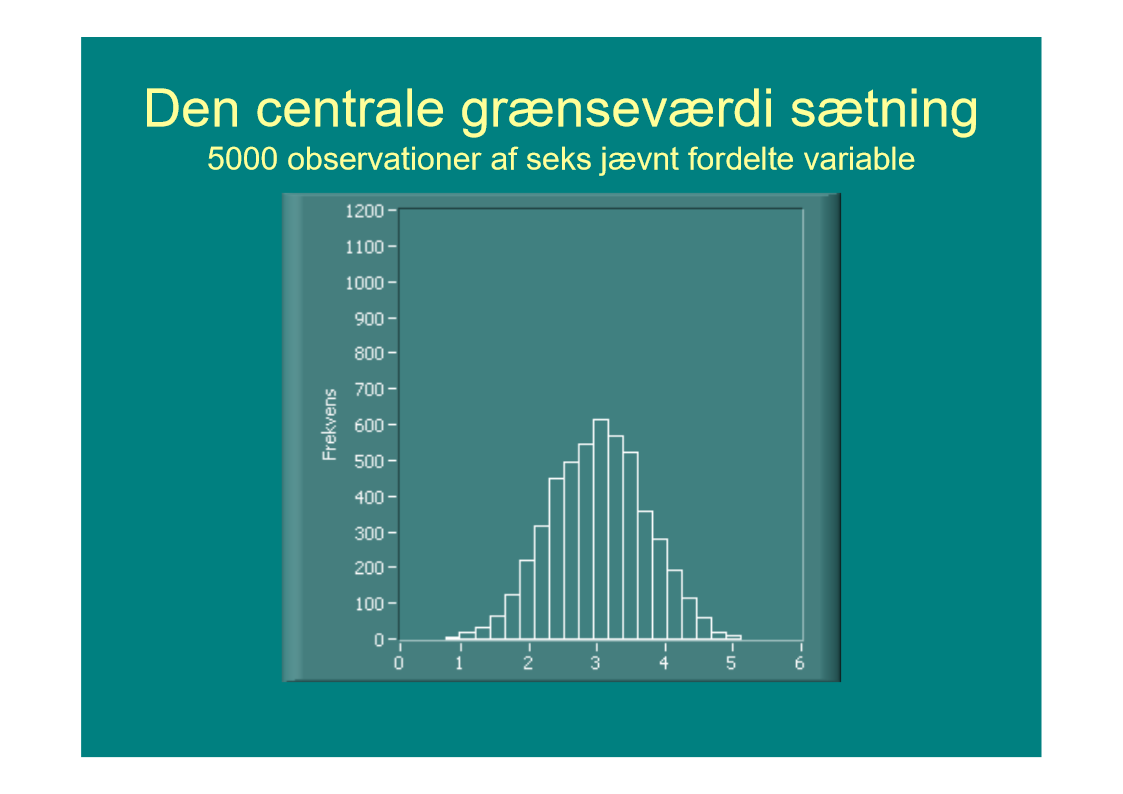
\includegraphics[width=\textwidth]{billeder/billede26}
\end{center}
Vil tilsidst blive til en normalfordeling jo mere de bliver summeret sammen (højere variable). 




\section{Transduerprincipper}

\begin{center}
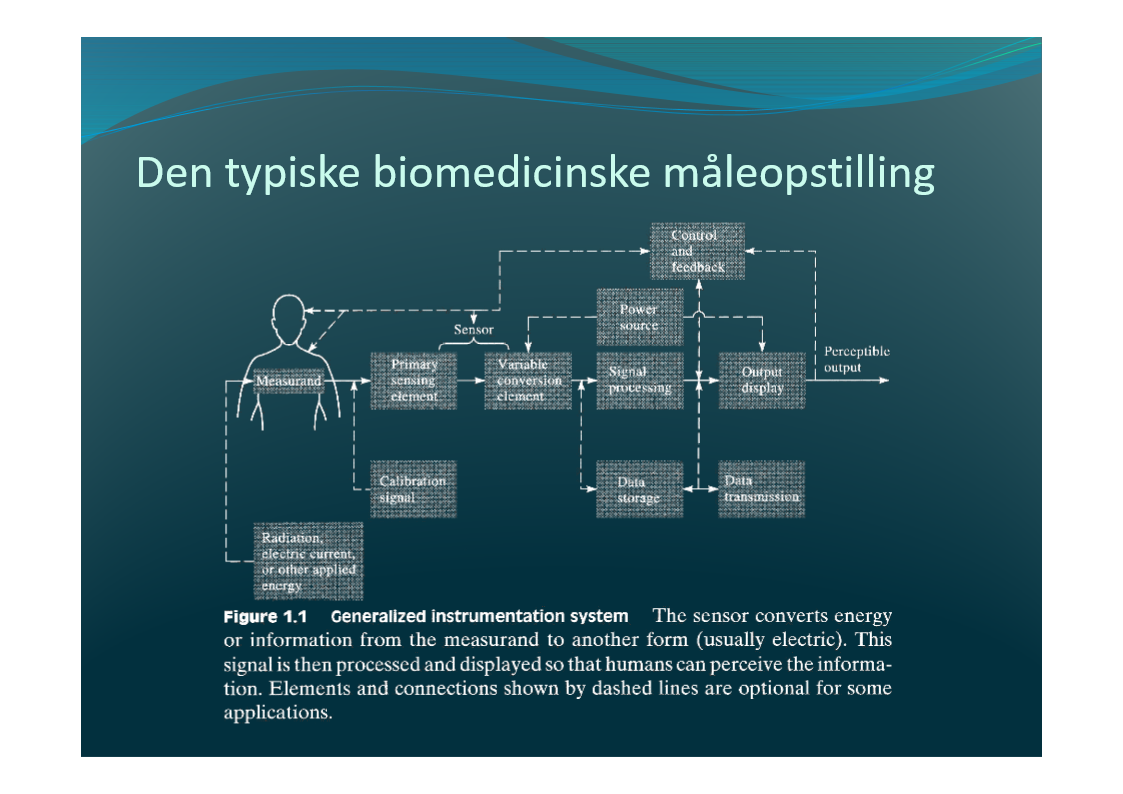
\includegraphics[width=\textwidth]{billeder/billede27}
\end{center}

\subsection{Resistive transducere}
\subsubsection{Potentiometer}
\begin{center}
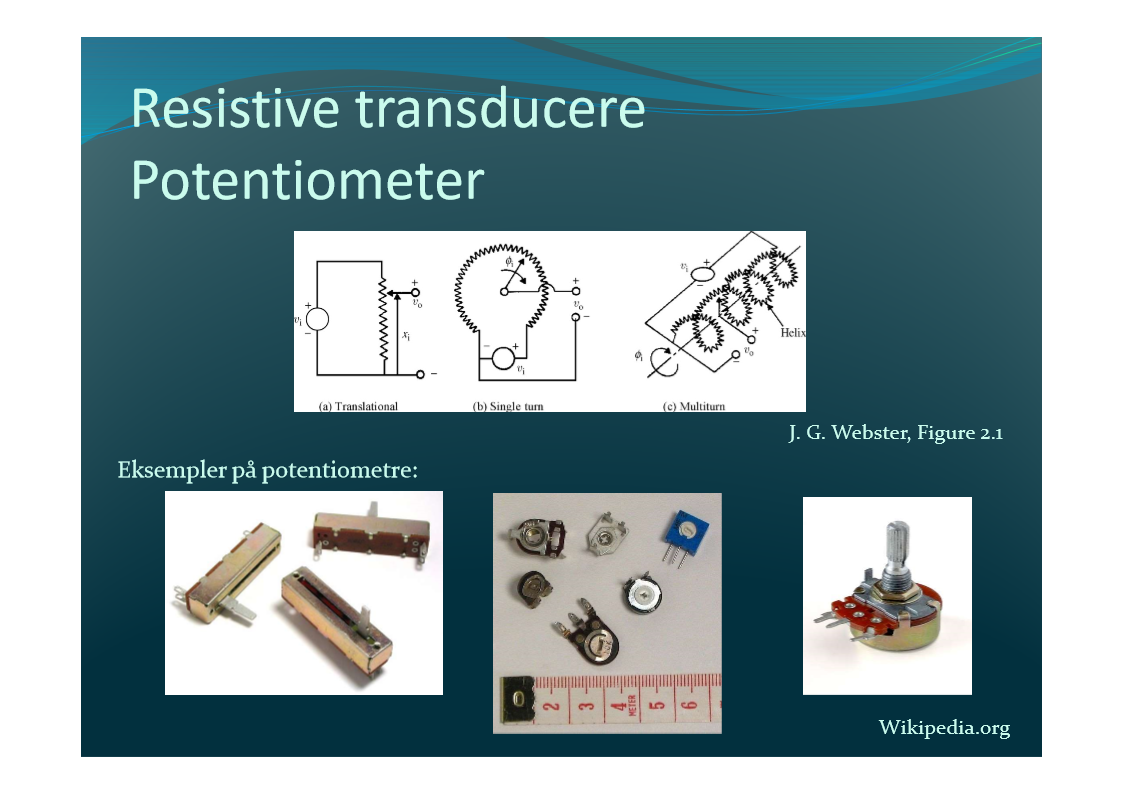
\includegraphics[width=\textwidth]{billeder/billede28}
\end{center}
Man kan sige at et potentiometer også kan kaldes for en spændingsdeler.

\begin{center}
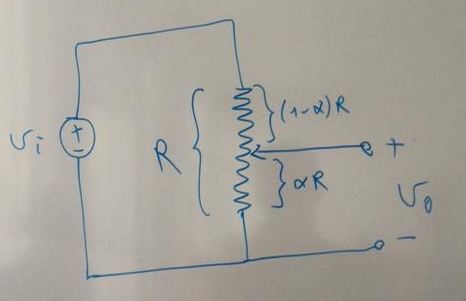
\includegraphics[width=\textwidth]{billeder/billede31}
\end{center}
$$v_0=\frac{\alpha*R}{R}*v_i = \alpha*v_i$$
Kan også bruges til at bestemme en vinkel med.






\newpage
\subsubsection{Strain gauges}

\begin{figure}[h!]
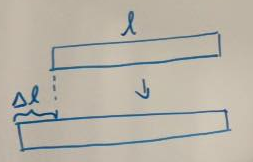
\includegraphics[width=\textwidth]{billeder/billede32}
\caption{En transformation}
\end{figure}

$$\epsilon = \frac{\Delta}L{L}$$
Hvor $\epsilon$ er vores strain.

\begin{center}
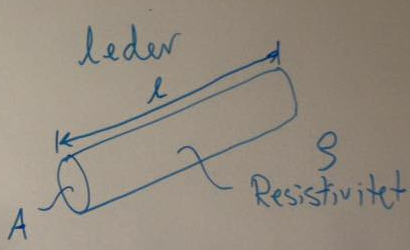
\includegraphics[width=\textwidth]{billeder/billede33}
\end{center}
$$R=\frac{l*\rho}{A}$$
Påvirkning af modstands værdien. Et lille areal, giver en stor modstand.
$$\frac{\partial*R}{\partial*\rho}=\frac{l}{A}\Rightarrow\partial*R_\partial=\frac{l*\partial*\rho}{A}$$





\begin{center}
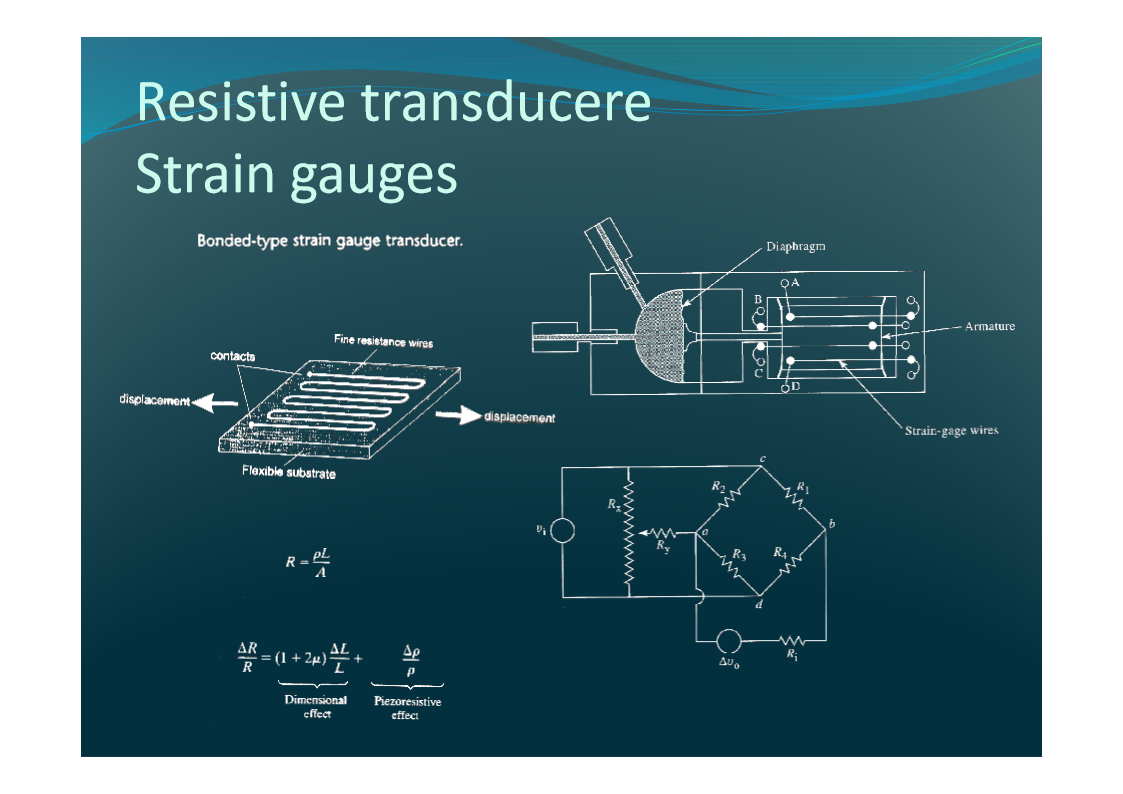
\includegraphics[width=\textwidth]{billeder/billede29}
\end{center}
En strain gauge er en modstandstråd som foldes og limes fast på et materiale som der så kan måles på. Det er strækningen vi gerne vil være i stand til at måle på, altså hvad bliver vores modstandsændring.


\begin{center}
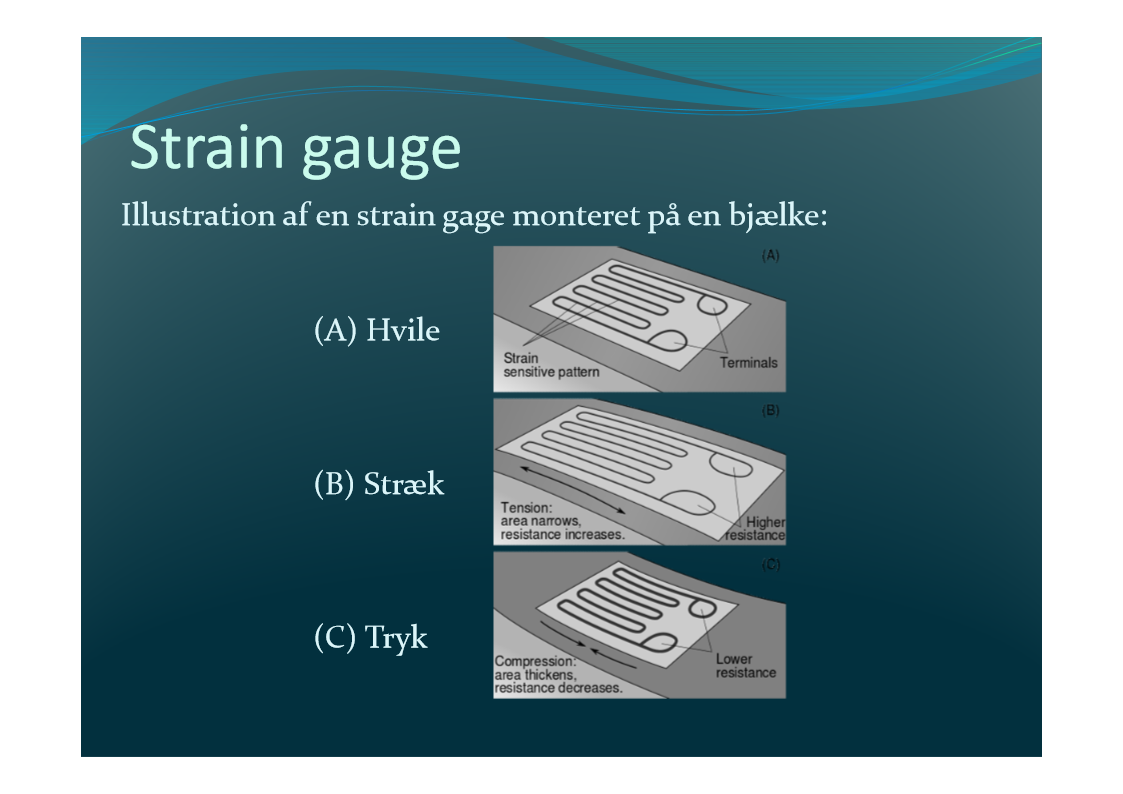
\includegraphics[width=\textwidth]{billeder/billede30}
\end{center}

Det er længden og tværsnitsarealet som ændre sig på strain gaugen og den bruges til følsomme målinger. Det kan f.eks være en måling fra en fysisk størrelse til et elektrisk signal eller et mekanisk tryk til et elektrisk signal.





\end{document}